\clearpage
\subsubsection{Case Statement} % (fold)
\label{sub:case_statement}

The case statement is the second kind of branching statement. This allows you to create paths that execute based on matching a value from an expression. This allows one case statement to handle many alternative paths.

\begin{figure}[h]
   \centering
   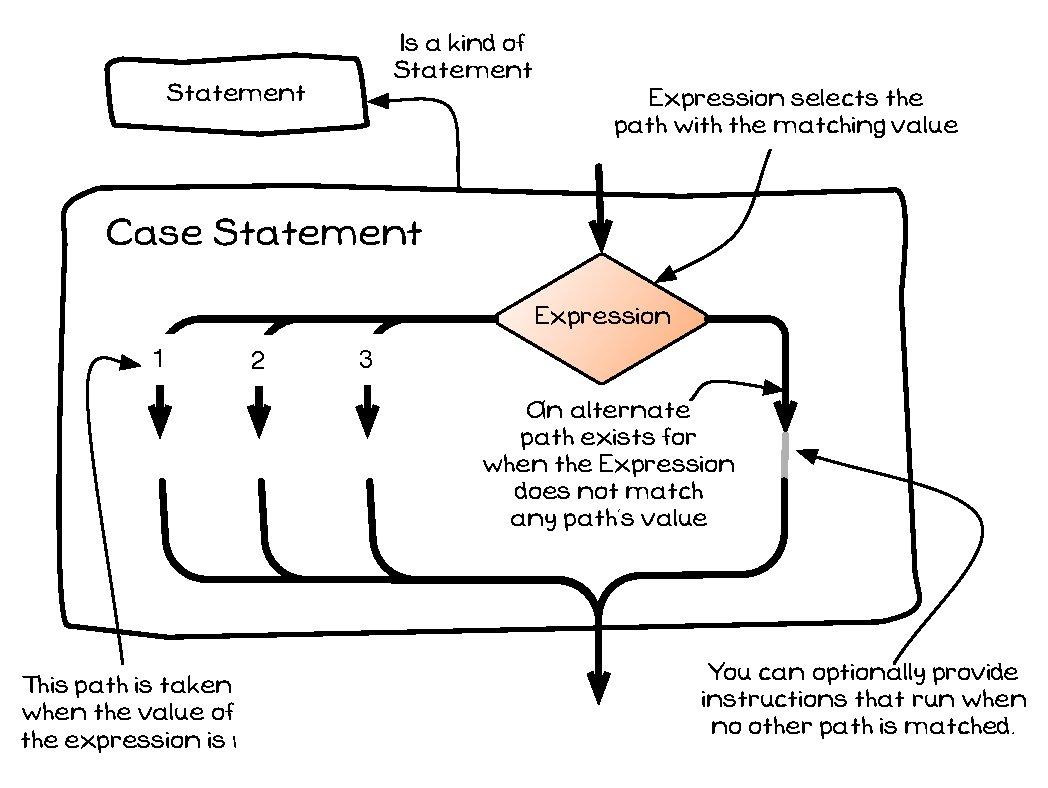
\includegraphics[width=\textwidth]{./topics/control-flow/diagrams/CaseStatement} 
   \caption{Case statement selectively runs multiple branches of code}
   \label{fig:branching-case-statement}
\end{figure}

\mynote{
\begin{itemize}
  \item The case statement is a kind of \textbf{action}. It allows you to command the computer to select a path based upon the value of an expression.
  \item Each path within the Case Statement has a value. When the computer executes the case statement the path values are used to determine which path will be taken.
  \item In C and Pascal the Case Statement only works with Ordinal Values. This limits you to using Character or Integer values within the Case Statement's Expression.
  \item The Case Statement has one entry point, multiple paths, and then one exit point.
\end{itemize}
}

% section case_statement (end)